% Source reference: :contentReference[oaicite:0]{index=0}
\part{Recurrence Relations}
\section{Handout 04: Recurrence Relations}

\subsection{Overview}

This handout begins Part II of the course. The goal is not yet to develop the full theory for solving recurrence relations, but to learn how to \emph{model} a problem recursively.

A recurrence relation is useful when a problem of size $n$ can be reduced to one or more smaller problems, typically of sizes $n-1$, $n-2$, and so on. In this handout, the emphasis is on:
\begin{itemize}[leftmargin=*]
    \item understanding what a recurrence relation is;
    \item identifying the correct size parameter;
    \item deriving initial conditions;
    \item splitting a problem into exhaustive and non-overlapping cases;
    \item relating a counting problem of size $n$ to smaller instances.
\end{itemize}

The main examples are:
\begin{itemize}[leftmargin=*]
    \item Tower of Hanoi;
    \item compound interest;
    \item the graduate-student job problem and Fibonacci numbers;
    \item $0$-$1$ strings with no consecutive $0$'s;
    \item decimal codewords with an even number of zero digits.
\end{itemize}

\begin{examtip}[title={Main objective of Handout 04}]
For this handout, the central task is usually not ``solve the recurrence completely'' but rather ``derive the correct recurrence and initial conditions.'' A recurrence is only useful if the state variable is defined precisely.
\end{examtip}

%==================================================
\subsection{What Is a Recurrence Relation?}
%==================================================

\begin{definition}{Recurrence relation and initial conditions}{recurrence-def}
A \emph{recurrence relation} for a sequence $(a_n)$ is an equation that expresses $a_n$ in terms of one or more earlier terms of the sequence.

The accompanying \emph{initial conditions} specify enough starting values to determine the sequence uniquely.
\end{definition}

A recurrence model usually has two parts:
\begin{enumerate}[leftmargin=*]
    \item define the quantity $a_n$ clearly in terms of the problem size $n$;
    \item relate the size-$n$ problem to smaller instances.
\end{enumerate}

\begin{keyformula}[title={Core modelling pattern}]
\[
\text{current value} = \text{contribution from smaller cases}.
\]
A valid recurrence model must also include initial conditions.
\end{keyformula}

\begin{examplebox}[title={A simple financial example}]
If $P_n$ denotes the amount in an account after $n$ years and the balance grows by $11\%$ each year, then
\[
P_n=1.11P_{n-1}
\]
with initial condition
\[
P_0=10{,}000.
\]
The recurrence comes from the rule that each year's balance is the previous year's balance plus $11\%$ of the previous year's balance.
\end{examplebox}

\begin{commonmistake}[title={A recurrence without initial conditions is incomplete}]
The formula
\[
a_n=a_{n-1}+a_{n-2}
\]
does not determine a unique sequence by itself. Different initial conditions produce different sequences.
\end{commonmistake}

%==================================================
\subsection{Idea of Recurrence}
%==================================================

The key idea is to solve a large problem by reducing it to smaller ones. For a problem parameterized by $n$, we try to answer:
\begin{center}
\emph{How can the size-$n$ case be built from cases of smaller size?}
\end{center}

Typical strategies include:
\begin{itemize}[leftmargin=*]
    \item removing the last object or last step;
    \item splitting according to the last symbol or first symbol;
    \item separating what is already present from what is newly created;
    \item introducing extra states when one variable does not capture enough information.
\end{itemize}

\begin{extension}[title={Recurrence modelling is structural, not computational}]
A good recurrence is obtained by understanding the \emph{structure} of the objects being counted. The equation is a consequence of that structure; it is not something guessed from a few numerical values.
\end{extension}

%==================================================
\subsection{Example: Tower of Hanoi}
%==================================================

Let $H_n$ denote the minimum number of moves needed to transfer $n$ disks from one bar to another, subject to the rules:
\begin{enumerate}[leftmargin=*]
    \item only one disk may be moved at a time;
    \item no disk may be placed on top of a smaller disk.
\end{enumerate}

\begin{examplebox}[title={Tower of Hanoi recurrence}]
Define $H_n$ to be the minimum number of moves required to transfer $n$ disks from one peg to another.

The initial condition is
\[
H_1=1.
\]

To move $n$ disks:
\begin{enumerate}[leftmargin=*]
    \item move the top $n-1$ disks to the spare peg: $H_{n-1}$ moves;
    \item move the largest disk: $1$ move;
    \item move the $n-1$ disks onto the largest disk: $H_{n-1}$ moves.
\end{enumerate}
Hence
\[
H_n=2H_{n-1}+1
\qquad (n\ge 2).
\]
\end{examplebox}

% Tower of Hanoi decomposition: move n-1, move largest, move n-1 again.
\begin{center}
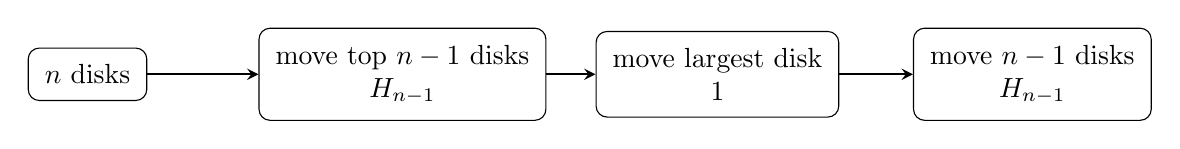
\begin{tikzpicture}[>=stealth]
    \node[draw,rounded corners,align=center,inner sep=6pt] (A) at (0,0) {$n$ disks};
    \node[draw,rounded corners,align=center,inner sep=6pt] (B) at (4.0,0) {move top $n-1$ disks\\$H_{n-1}$};
    \node[draw,rounded corners,align=center,inner sep=6pt] (C) at (8.0,0) {move largest disk\\$1$};
    \node[draw,rounded corners,align=center,inner sep=6pt] (D) at (12.0,0) {move $n-1$ disks\\$H_{n-1}$};
    \draw[->,thick] (A) -- (B);
    \draw[->,thick] (B) -- (C);
    \draw[->,thick] (C) -- (D);
\end{tikzpicture}
\end{center}

One can compute the first few values:
\[
H_1=1,\quad H_2=3,\quad H_3=7,\quad H_4=15,\quad H_5=31.
\]
This suggests the closed form
\[
H_n=2^n-1.
\]
Indeed, this can be proved by induction:
\[
H_n=2H_{n-1}+1=2(2^{n-1}-1)+1=2^n-1.
\]

\begin{examtip}[title={Why this recurrence is natural}]
The largest disk can move only once the top $n-1$ disks have been cleared, and after that those $n-1$ disks must be rebuilt on top of it. This forces the decomposition
\[
H_n=H_{n-1}+1+H_{n-1}.
\]
\end{examtip}

\begin{extension}[title={Reve's puzzle}]
If there are $k\ge 4$ pegs instead of $3$, the problem becomes a much deeper one. The four-peg case was solved only recently, and the general closed-form problem for larger $k$ is far subtler than the classical three-peg recurrence.
\end{extension}

%==================================================
\subsection{Example: Compound Interest}
%==================================================

\begin{examplebox}[title={Compound interest recurrence}]
Suppose $10{,}000$ dollars are deposited into an account earning $11\%$ annual interest, compounded once per year. Let $P_n$ denote the amount after $n$ years.

Then
\[
P_0=10{,}000,
\qquad
P_n=P_{n-1}+0.11P_{n-1}=1.11P_{n-1}.
\]
Iterating gives
\[
P_1=1.11P_0,
\qquad
P_2=1.11P_1=(1.11)^2P_0,
\qquad
\dots,
\qquad
P_n=(1.11)^nP_0.
\]
Hence
\[
P_{30}=(1.11)^{30}\cdot 10{,}000\approx 228{,}922.97.
\]
\end{examplebox}

This example is important because the recurrence is immediate from the problem statement. It also shows that some recurrences are simple enough to solve by direct iteration.

\begin{commonmistake}[title={Confusing the recurrence with the final closed form}]
The recurrence
\[
P_n=1.11P_{n-1}
\]
is the model. The expression
\[
P_n=(1.11)^nP_0
\]
is a derived formula obtained by repeated substitution.
\end{commonmistake}

%==================================================
\subsection{Example: Graduate-Student Job Problem}
%==================================================

Consider the following model: each professor graduates one student every year who becomes a professor, except first-year professors, who graduate no students. Assume no retirements.

Let $f_n$ denote the number of professors in year $n$.

The initial values are
\[
f_0=0,\qquad f_1=1,\qquad f_2=1.
\]
The first few values are
\[
f_3=2,\qquad f_4=3,\qquad f_5=5.
\]

\begin{examplebox}[title={Graduate-student job recurrence}]
To count the professors in year $n$, split them into two groups:
\begin{itemize}[leftmargin=*]
    \item the professors already present in year $n-1$, contributing $f_{n-1}$;
    \item the new professors produced in year $n$, which come from those who were already beyond their first year in year $n-1$.
\end{itemize}
These new professors correspond exactly to the professors present in year $n-2$. Therefore
\[
f_n=f_{n-1}+f_{n-2}
\qquad (n\ge 2).
\]
\end{examplebox}

This is the Fibonacci recurrence. The sequence $(f_n)$ is therefore the Fibonacci sequence with the given initial conditions.

\begin{extension}[title={Same recurrence, different initial conditions}]
The recurrence
\[
a_n=a_{n-1}+a_{n-2}
\]
appears in many unrelated problems. What distinguishes one application from another is often the initial conditions. Later in this handout, the same recurrence will appear again in a string-counting problem.
\end{extension}

%==================================================
\subsection{Example: Bit Strings With No Consecutive Zeros}
%==================================================

Let $a_n$ denote the number of $0$-$1$ strings of length $n$ that do not contain two consecutive $0$'s.

The initial values are
\[
a_1=2
\qquad\text{(namely $0,1$)},
\qquad
 a_2=3
\qquad\text{(namely $01,10,11$)}.
\]

\begin{examplebox}[title={Recurrence for strings with no consecutive zeros}]
Consider a valid string of length $n$ and examine its last bit.

\textbf{Case 1:} The last bit is $1$.
Then the first $n-1$ bits may be any valid string of length $n-1$. Hence this case contributes
\[
a_{n-1}.
\]

\textbf{Case 2:} The last bit is $0$.
Then the $(n-1)$st bit must be $1$, so the first $n-2$ bits may be any valid string of length $n-2$. Hence this case contributes
\[
a_{n-2}.
\]

The two cases are disjoint and exhaustive, so
\[
a_n=a_{n-1}+a_{n-2}
\qquad (n\ge 3).
\]
\end{examplebox}

% Case split for the final bit in a valid binary string with no consecutive zeros.
\begin{center}
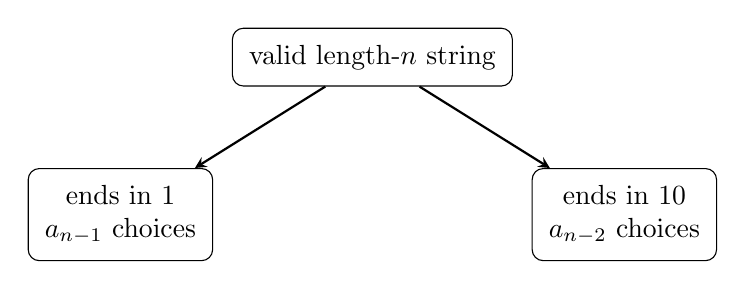
\begin{tikzpicture}[>=stealth]
    \node[draw,rounded corners,align=center,inner sep=6pt] (A) at (0,0) {valid length-$n$ string};
    \node[draw,rounded corners,align=center,inner sep=6pt] (B) at (-3.2,-2.0) {ends in $1$\\$a_{n-1}$ choices};
    \node[draw,rounded corners,align=center,inner sep=6pt] (C) at (3.2,-2.0) {ends in $10$\\$a_{n-2}$ choices};
    \draw[->,thick] (A) -- (B);
    \draw[->,thick] (A) -- (C);
\end{tikzpicture}
\end{center}

Thus $(a_n)$ satisfies the same recurrence as the Fibonacci numbers, but with different initial conditions.

\begin{examtip}[title={Standard last-symbol strategy}]
When deriving a recurrence for strings, examining the last symbol is often the cleanest approach. The key is to ensure that the resulting cases are both exhaustive and disjoint.
\end{examtip}

%==================================================
\subsection{Example: Decimal Codewords With an Even Number of Zeros}
%==================================================

A decimal string is a valid codeword if it contains an even number of zero digits. Let $a_n$ denote the number of valid codewords of length $n$.

\begin{examplebox}[title={Codeword recurrence via last digit}]
Consider a codeword of length $n$ and inspect its last digit.

\textbf{Case 1:} The last digit is nonzero.
There are $9$ choices for this digit, and the preceding $n-1$ digits must already form a valid codeword. Hence this case contributes
\[
9a_{n-1}.
\]

\textbf{Case 2:} The last digit is $0$.
Then the preceding $n-1$ digits must contain an \emph{odd} number of zeros. The total number of decimal strings of length $n-1$ is $10^{n-1}$, and among these, exactly $a_{n-1}$ have an even number of zeros. Therefore the number with an odd number of zeros is
\[
10^{n-1}-a_{n-1}.
\]
Hence this case contributes
\[
10^{n-1}-a_{n-1}.
\]

Adding the two cases gives
\[
a_n=9a_{n-1}+(10^{n-1}-a_{n-1})=8a_{n-1}+10^{n-1}.
\]
\end{examplebox}

A convenient initial condition is
\[
a_0=1,
\]
since the empty string contains $0$ zeros, which is even. Equivalently, one may use
\[
a_1=9.
\]

% Even/odd parity transition diagram for the number of 0-digits.
\begin{center}
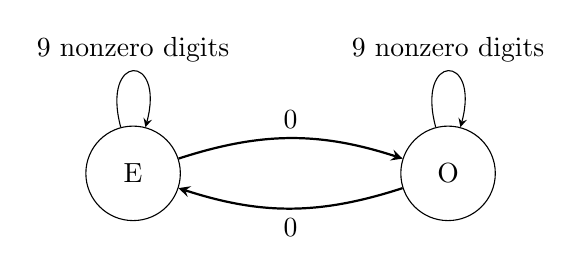
\begin{tikzpicture}[>=stealth]
    \node[draw,circle,minimum size=1.2cm] (E) at (0,0) {E};
    \node[draw,circle,minimum size=1.2cm] (O) at (4,0) {O};
    \draw[->,loop above] (E) to node[above] {$9$ nonzero digits} (E);
    \draw[->,loop above] (O) to node[above] {$9$ nonzero digits} (O);
    \draw[->,bend left=18,thick] (E) to node[above] {$0$} (O);
    \draw[->,bend left=18,thick] (O) to node[below] {$0$} (E);
\end{tikzpicture}
\end{center}

\begin{extension}[title={State augmentation viewpoint}]
This example shows that a single quantity may be insufficient unless the state captures the right information. Here the relevant hidden state is the \emph{parity} of the number of zeros. One may track even and odd states separately, then eliminate the odd state to obtain a one-variable recurrence.
\end{extension}

\begin{commonmistake}[title={Forgetting the complement count}]
In the zero-ending case, the preceding string must have an odd number of zeros, not an even number. The handout avoids introducing a second sequence by counting the odd case as
\[
10^{n-1}-a_{n-1}.
\]
\end{commonmistake}

%==================================================
\subsection{What This Handout Does Not Yet Do}
%==================================================

Handout 04 focuses on \emph{forming} recurrences and identifying initial conditions. Systematic methods for solving more general recurrence relations are deferred to Handouts 05 and 06.

\begin{examtip}[title={Scope boundary}]
In this handout, deriving the recurrence correctly is the main objective. When a closed form is not immediate, it is acceptable to stop once the recurrence and initial data have been obtained clearly.
\end{examtip}

%==================================================
\subsection{Special Techniques}
%==================================================

\subsubsection*{1. Define the state precisely}
A recurrence begins with a precise quantity. State clearly what $a_n$ counts or measures, and what the size parameter $n$ means.

\subsubsection*{2. Split by the last step or last symbol}
For process problems, inspect the final move. For strings, inspect the last symbol. This often produces natural disjoint cases.

\subsubsection*{3. Separate old contribution from new contribution}
In growth models, write the current total as
\[
\text{previous total} + \text{new amount added now}.
\]
This is the key idea in the graduate-student job problem.

\subsubsection*{4. Use complement counting when a second state is awkward}
In the codeword example, the odd-zero case is counted as
\[
10^{n-1}-a_{n-1}
\]
instead of introducing a second recurrence immediately.

\subsubsection*{5. Compare with known sequences carefully}
Two different problems may satisfy the same recurrence. Do not conclude that the sequences are identical until the initial conditions are also checked.

\subsubsection*{6. Compute a few early terms as a plausibility check}
Before trusting a recurrence, calculate the first few values manually. This helps detect missing cases or incorrect initial conditions.

\begin{extension}[title={A robust recurrence-building workflow}]
For a new problem, try the following order:
\begin{enumerate}[leftmargin=*]
    \item choose the parameter $n$;
    \item define the state variable precisely;
    \item classify size-$n$ objects into natural disjoint cases;
    \item express each case in terms of smaller sizes;
    \item write initial conditions separately;
    \item test the recurrence on small values.
\end{enumerate}
\end{extension}

%==================================================
\subsection{Summary Table}
%==================================================

\begin{center}
\small
\begin{tabular}{@{}p{0.30\textwidth}p{0.29\textwidth}p{0.29\textwidth}@{}}
\toprule
\textbf{Problem} & \textbf{State variable} & \textbf{Recurrence / data} \\
\midrule
Tower of Hanoi & $H_n$ = minimum moves for $n$ disks & $H_1=1$, \\ $H_n=2H_{n-1}+1$ \\
Compound interest & $P_n$ = amount after $n$ years & $P_0=10{,}000$, \\ $P_n=1.11P_{n-1}$ \\
Graduate-student job problem & $f_n$ = number of professors in year $n$ & $f_0=0$, $f_1=1$, \\ $f_n=f_{n-1}+f_{n-2}$ \\
No consecutive zeros & $a_n$ = valid bit strings of length $n$ & $a_1=2$, $a_2=3$, \\ $a_n=a_{n-1}+a_{n-2}$ \\
Even number of zero digits & $a_n$ = valid decimal codewords of length $n$ & $a_0=1$, \\ $a_n=8a_{n-1}+10^{n-1}$ \\
\bottomrule
\end{tabular}
\end{center}

\begin{commonmistake}[title={Final warning for Handout 04}]
A recurrence is not obtained by observing a pattern in a few numerical values alone. The recurrence must come from a mathematically justified decomposition of the problem into smaller cases.
\end{commonmistake}